\documentclass[DIV=calc, paper=a4, fontsize=11pt]{scrartcl}


\usepackage{makeidx}
\usepackage{graphicx}
\usepackage{flushend}

\usepackage{lmodern}
\usepackage[left=1.5cm,right=1.5cm,top=2.5cm,bottom=2cm]{geometry}
\usepackage{float}		
\bibliographystyle{plain} 
\pagestyle{plain} 
\pagenumbering{arabic}
\usepackage{fancyhdr} 	


\usepackage[T1]{fontenc}
\usepackage[utf8]{inputenc}
\usepackage[spanish]{babel}
\usepackage{hyperref}
\usepackage{graphicx}

\usepackage{lipsum}
\usepackage[protrusion=true,expansion=true]{microtype}
\usepackage{amsmath,amsfonts,amsthm}
\usepackage[svgnames]{xcolor}
\usepackage[svgnames]{xcolor}
\usepackage{booktabs}
\usepackage{fix-cm}
\usepackage{multicol}
\newenvironment{Figura}
  {\par\medskip\noindent\minipage{\linewidth}}
  {\endminipage\par\medskip}

\usepackage{sectsty}
\usepackage{siunitx}
\allsectionsfont{\usefont{OT1}{phv}{b}{n}}

\usepackage{fancyhdr}
\pagestyle{fancy}
\usepackage{lastpage}

\lhead{}
\chead{}
\rhead{}

\lfoot{}
\cfoot{}
\rfoot{\footnotesize Page \thepage\ of \pageref{LastPage}}

\renewcommand{\headrulewidth}{0.0pt}
\renewcommand{\footrulewidth}{0.4pt}

\usepackage{lettrine}
\newcommand{\initial}[1]{\lettrine[lines=3,lhang=0.3,nindent=0em]{
\color{DarkGoldenrod}{\textsf{#1}}}{}}

\usepackage{titling}

\newcommand{\HorRule}{\color{DarkGoldenrod} \rule{\linewidth}{1pt}}

\pretitle{\vspace{-120pt} \begin{flushleft} \HorRule \fontsize{22}{35} \usefont{OT1}{phv}{b}{n} \color{DarkRed} \selectfont}

\title{Viscosidad\\ %Aquí va el nombre de la práctica 
Práctica 5} %Numero de la práctica 

\posttitle{\par\end{flushleft}\vskip 0.5em}

\preauthor{\begin{flushleft}\large \lineskip 0.5em \usefont{OT1}{phv}{b}{sl} \color{DarkRed}}

\author{Misael Iván Macías Márquez\\
misaelmacias@ciencias.unam.mx}

\postauthor{\footnotesize \usefont{OT1}{phv}{m}{sl} \color{Black}

\vspace*{0.1cm} Facultad de Ciencias, UNAM

\par\end{flushleft}\HorRule}

\date{Miércoles 20 de Abril de 2022\\Semestre 2022-2}


\begin{document}

\maketitle


\begin{abstract}
\textbf{Resumen:} Se determinaron los coeficientes de viscosidad para el shampoo, agua y glicerina haciendo uso de datos recabados por otros grupos de alumnos. Los coeficientes de viscosidad obtenidos son $(50 \pm 15000)\frac{kg}{ms}$, $(116 \pm 824) \frac{kg}{ms}$ y $(9 \pm 2600) \frac{kg}{ms}$ para el shampoo, agua y glicerina respectivamente. Los resultados fueron tanto imprecisos como inexactos.
\end{abstract}

\begin{multicols}{2}




\section*{Introducción}

La viscosidad es fricción interna en un fluido. Las fuerzas viscosas se oponen al movimiento de una parte de un fluido en relación con otra. La viscosidad es la razón por la que se dificulta remar una canoa en aguas tranquilas, pero también es lo que hace que funcione el remo. Los efectos de la viscosidad son importantes en el flujo de fluidos en las tuberías, en el flujo de la sangre, en la lubricación de las partes de un motor y en muchas otras situaciones[1].

De la ley de Stokes con el cuerpo que se mueve en el fluido una esfera, tenemos[2]

\begin{equation*}
    F_r = 6 \pi R \eta v_f
\end{equation*}

donde $F_r$ es la fuerza de resistencia del fluido, $R$ el radio de la esfera sumergida, $\eta$ el coeficiente de viscosidad y $v_f$ la velocidad final del cuerpo en el fluido[2].

Haciendo el diagrama de fuerzas donde participan el empuje $E$, la fuerza de resistencia $F_r$ y la fuerza de gravedad $F_g$, y posteriormente despejando $\eta$ se tiene[2]



\begin{equation}
    \eta = \frac{2R^2 g(\rho_e - \rho_f)}{9 v_f}
\end{equation}

donde $\rho_e$ es la densidad de la esfera y $\rho_f$ es la densidad del fluido.



\section*{Desarrollo experimental}

\begin{Figura}
\centering
    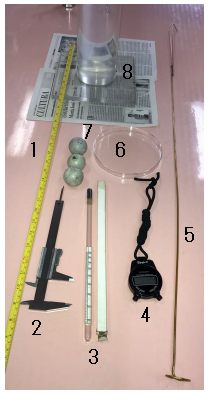
\includegraphics[width=0.8\textwidth]{viscosidad 1.PNG}
    \captionof{figure}{Material:  (1) flexometro, (2) vernier, (3) Densímetro, (4) cronometro, (5) varilla, (6) mitad de caja petri, (7) pelotas con distintas características, (8) Probeta grande}
    \label{fig}
\end{Figura}

\begin{Figura}
\centering
    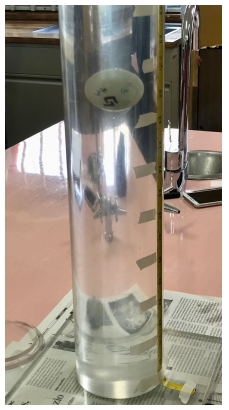
\includegraphics[width=0.8\textwidth]{viscosidad 2.PNG}
    \captionof{figure}{Montaje experimental.}
    \label{fig}
\end{Figura}

La práctica fue realizada por otro grupo de estudiantes, su desarrollo experimental es el siguiente:

\begin{enumerate}

    \item Con ayuda del densímetro obtener la densidad del fluido de la primer probeta.

    \item Usando el vernier, medir los diámetros de las 3 pelotas y con ayuda de la báscula digital pesar cada una de ellas.
    
    \item Graduar la probeta con ayuda de cinta adhesiva cada 5 cm.
    
    \item Dejar caer cada una de las pelotas en el fluido de la probeta, y con un cronómetro medir el tiempo que tarda en recorrer cada marca, repetir este procedimiento 5 veces para cada una de las pelotas, figura (2).
    
    \item Repetir el paso anterior con las otras dos pelotas.
    
    \item Repetir todos los pasos anteriores para cada probeta.
\end{enumerate}



\section*{Resultados y análisis}

La densidad de una esfera de radio $R$ con masa $m$ es:

\begin{equation*}
    \rho_e = \frac{m}{\frac{3}{4}\pi R^3 }
\end{equation*}

con una incertidumbre de 

\begin{equation*}
    \delta \rho_e = \sqrt{\left(\frac{\partial \rho_e}{\partial m}\delta m\right)^{2}+ \left(\frac{\partial \rho_e}{\partial R}\delta 
    R\right)^2}
\end{equation*}

\begin{equation*}
    =\frac{1}{R^3}\sqrt{\left(\frac{4 \delta m}{3\pi}\right)^{2}+\left(\frac{3m\delta R}{R}\right)^{2}}
\end{equation*}

Las esferas usadas son, la pelota 1 de masa $91.1g$ y radio $1.53cm$, pelota 2 de masa $47.2g$ y radio $1.53cm$, pelota 3 de masa $48.6g$ y radio $1.53cm$ y pelota 4 de masa $64.1g$ y radio $1.99cm$. Sus densidades son:

\begin{equation*}
    \rho_{e1} = (10795.2561 \pm 999.1920) \frac{kg}{m^3}
\end{equation*}

\begin{equation*}
    \rho_{e2} = (3146.1477 \pm 520.1038) \frac{kg}{m^3}
\end{equation*}

\begin{equation*}
    \rho_{e3} = (3239.4656 \pm 535.3384) \frac{kg}{m^3}
\end{equation*}

\begin{equation*}
    \rho_{e4} = (3452.1342 \pm 248.4621) \frac{kg}{m^3}
\end{equation*}

Las densidades de los fluidos usados son:

\begin{equation*}
    \rho_{s}= (1120 \pm 0.00005) \frac{kg}{m^3}
\end{equation*}

\begin{equation*}
    \rho_{a} = (1000 \pm 0.00005) \frac{kg}{m^3}
\end{equation*}

\begin{equation*}
    \rho_{g} = (1240 \pm 0.00005) \frac{kg}{m^3}
\end{equation*}



Propagando la incertidumbre de la ecuación (1)

\begin{equation*}
    \delta \eta = \sqrt{\left(\frac{\partial \eta}{\partial R}\delta R\right)^{2} + \left(\frac{\partial \eta}{\partial  \rho_e} \delta \rho_{e}\right)^{2} + \left(\frac{\partial \eta}{\partial  \rho_f} \delta \rho_f \right)^{2} + \left(\frac{\partial \eta}{\partial  v_f} \delta v_f\right)^{2}}
\end{equation*}

y no hay suficiente espacio así que lo pondré en un pie de pagina\footnote{$= \frac{2R g}{v_f} \sqrt{(\rho_e - \rho_f)^2\left[\left(\frac{2}{9}\delta R\right)^2+\left(\frac{R}{v_f}\delta v_f\right)^2\right] +\frac{R^2}{9^2} \left[\left(\rho_f \delta \rho_e\right)^{2} + \left(\rho_e \delta \rho_f\right)^{2}\right]}$}.



\subsection*{Shampoo}

\begin{Figura}
\centering
    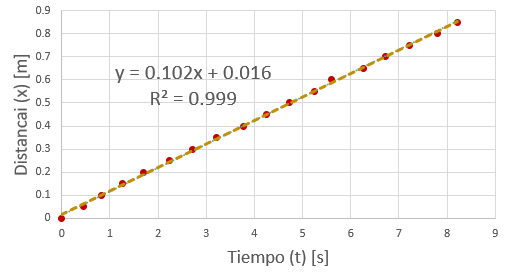
\includegraphics[width=1\textwidth]{graficas/1 shampoo.PNG}
    \captionof{figure}{Gráfica de ajuste para determinar la velocidad final para la pelota 1 en el shampoo.}
    \label{fig}
\end{Figura}

La velocidad final obtenida para la pelota 1 en el shampoo es:

\begin{equation*}
    v_f = (0.102 \pm 0.001) \frac{m}{s}
\end{equation*}

lo que nos da un coeficiente de viscosidad para el shampoo de:

\begin{equation*}
    \eta_{s} = (48.367 \pm 5594.377) \frac{kg}{ms}
\end{equation*}


\begin{Figura}
\centering
    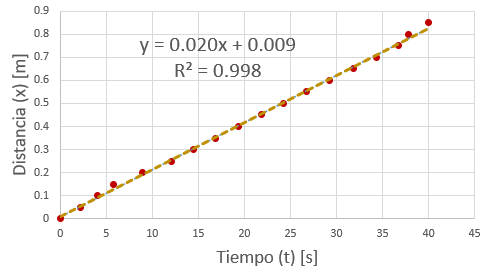
\includegraphics[width=1\textwidth]{graficas/2 shampoo.PNG}
    \captionof{figure}{Gráfica de ajuste para determinar la velocidad final para la pelota 2 en el shampoo.}
    \label{fig}
\end{Figura}

La velocidad final obtenida para la pelota 2 en el shampoo es:

\begin{equation*}
    v_f = (0.020 \pm 0.001) \frac{m}{s}
\end{equation*}

lo que nos da un coeficiente de viscosidad para el shampoo de:

\begin{equation*}
    \eta_{s} = (50.549 \pm 14556.974) \frac{kg}{ms}
\end{equation*}

promediando y sumando por cuadraturas las incertidumbres tenemos un coeficiente de viscosidad final de:

\begin{equation*}
    \eta_{s} = (50 \pm 15000) \frac{kg}{ms} 
\end{equation*}

el coeficiente reportado en la literatura es $(1.25 - 9)\frac{kg}{ms}$.

\subsection*{Agua}

\begin{Figura}
\centering
    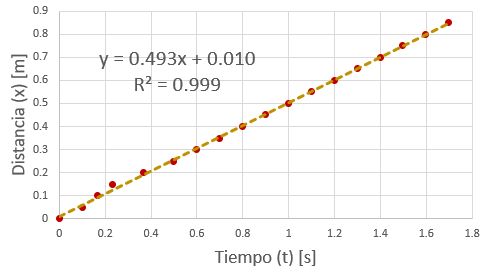
\includegraphics[width=1\textwidth]{graficas/2 agua.PNG}
    \captionof{figure}{Gráfica de ajuste para determinar la velocidad final para la pelota 2 en el agua.}
    \label{fig}
\end{Figura}

La velocidad final obtenida para la pelota 2 en el agua es:

\begin{equation*}
    v_f = (0.493 \pm 0.004) \frac{m}{s}
\end{equation*}

lo que nos da un coeficiente de viscosidad para el agua de:

\begin{equation*}
    \eta_{a} = (2.221 \pm 602.704) \frac{kg}{ms}
\end{equation*}

\begin{Figura}
\centering
    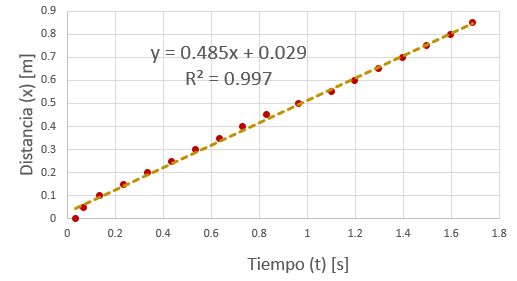
\includegraphics[width=1\textwidth]{graficas/3 agua.PNG}
    \captionof{figure}{Gráfica de ajuste para determinar la velocidad final para la pelota 3 en el agua.}
    \label{fig}
\end{Figura}

La velocidad final obtenida para la pelota 3 en el agua es:

\begin{equation*}
    v_f = (0.485 \pm 0.007) \frac{m}{s}
\end{equation*}

lo que nos da un coeficiente de viscosidad para el agua de:

\begin{equation*}
    \eta_{a} = (229.381 \pm 563.050) \frac{kg}{ms}
\end{equation*}

promediando y sumando por cuadraturas las incertidumbres tenemos un coeficiente de viscosidad final de:

\begin{equation*}
    \eta_{a} = (116 \pm 824 ) \frac{kg}{ms}
\end{equation*}

el coeficiente reportado en la literatura es $0.00105 \frac{kg}{ms}$.


\subsection*{Glicerina}

\begin{Figura}
\centering
    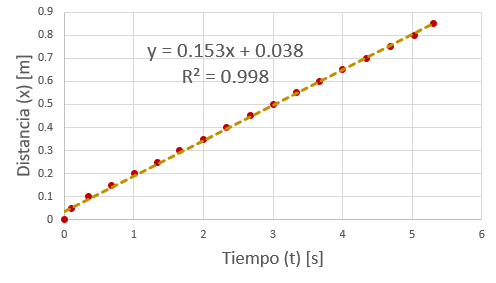
\includegraphics[width=1\textwidth]{graficas/2 glicerina.PNG}
    \captionof{figure}{Gráfica de ajuste para determinar la velocidad final para la pelota 2 en glicerina.}
    \label{fig}
\end{Figura}

La velocidad final obtenida para la pelota 2 en el glicerina es:

\begin{equation*}
    v_f = (0.153 \pm 0.002) \frac{m}{s}
\end{equation*}

lo que nos da un coeficiente de viscosidad para glicerina de:

\begin{equation*}
    \eta_{g} = (6.347 \pm 1939.724) \frac{kg}{ms}
\end{equation*}


\begin{Figura}
\centering
    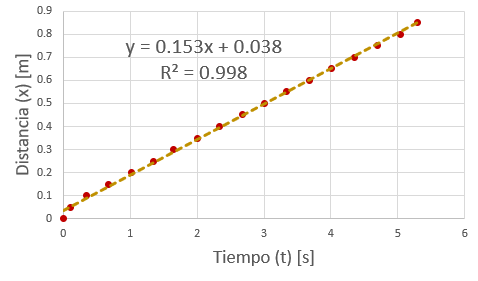
\includegraphics[width=1\textwidth]{graficas/4 glicerina.PNG}
    \captionof{figure}{Gráfica de ajuste para determinar la velocidad final para la pelota 4 en glicerina.}
    \label{fig}
\end{Figura}

La velocidad final obtenida para la pelota 4 en el glicerina es:

\begin{equation*}
    v_f = (0.153 \pm 0.002) \frac{m}{s}
\end{equation*}

lo que nos da un coeficiente de viscosidad para glicerina de:

\begin{equation*}
    \eta_{g} = (12.461 \pm 1735.550) \frac{kg}{ms}
\end{equation*}

promediando y sumando por cuadraturas las incertidumbres tenemos un coeficiente de viscosidad final de:

\begin{equation*}
    \eta_{g} = (9 \pm 2600 ) \frac{kg}{ms}
\end{equation*}

el coeficiente reportado en la literatura es $1.39 \frac{kg}{ms}$.

\section*{Conclusiones}

Los rangos obtenidos para los coeficientes de viscosidad para el shampoo, agua y glicerina , aunque incluyen los valores teóricos reportados en la literatura, son completamente imprecisos y exactos por lo que no se pueden considerar satisfactorios, este error podría deberse a un mal manejo en la propagación de incertidumbres y también posiblemente errores cometidos en el desarrollo experimental.
  
\begin{thebibliography}{99}
\bibitem{1} Sears, Zemansky Física universitaria Vol. 1, Gpo.
Edit. Pearson Educación, 12 ed.l, México, 2009.

\bibitem{1} https://moodle.fciencias.unam.mx/cursos/pluginfile.php/

151807/mod$_$resource/content/1/P7\%20Viscosidad.pdf

\end{thebibliography}

\section*{Apéndices}

\subsection*{Tablas}

\subsubsection*{grupo A}

\begin{Figura}
\centering
    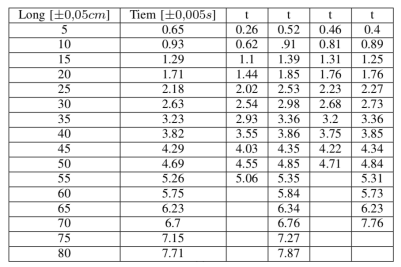
\includegraphics[width=0.8\textwidth]{tablas/tabla 1 viscosidad.PNG}
    \captionof{table}{Datos obtenidos para el Shampoo con la pelota 1, cada columna t representa una de las 5 distintas corridas de datos.}
    \label{fig}
\end{Figura}

\begin{Figura}
\centering
    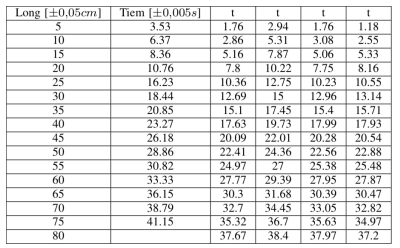
\includegraphics[width=0.8\textwidth]{tablas/tabla 2 viscosidad.PNG}
    \captionof{table}{Datos obtenidos para el Shampoo con la pelota 2, cada columna t representa una de las 5 distintas corridas de datos.}
    \label{fig}
\end{Figura}

\begin{Figura}
\centering
    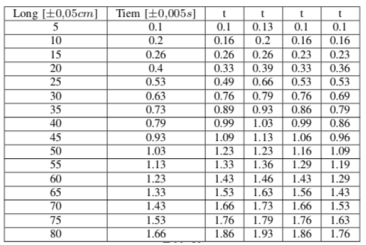
\includegraphics[width=0.8\textwidth]{tablas/tabla 3 viscosidad.PNG}
    \captionof{table}{Datos obtenidos para el agua con la pelota 2, cada columna t representa una de las 5 distintas corridas de datos.}
    \label{fig}
\end{Figura}

\begin{Figura}
\centering
    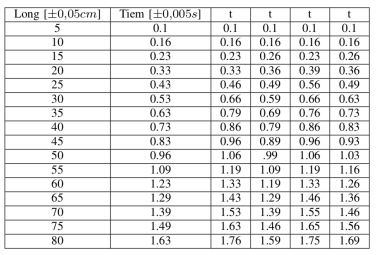
\includegraphics[width=0.8\textwidth]{tablas/tabla 4 viscosidad.PNG}
    \captionof{table}{Datos obtenidos para el agua con la pelota 3, cada columna t representa una de las 5 distintas corridas de datos.}
    \label{fig}
\end{Figura}

\begin{Figura}
\centering
    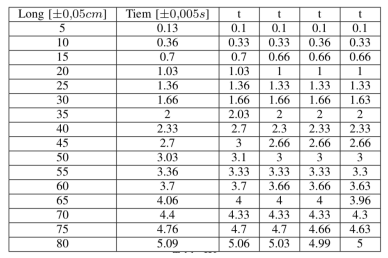
\includegraphics[width=0.8\textwidth]{tablas/tabla 5 viscosidad.PNG}
    \captionof{table}{Datos obtenidos para el glicerina con la pelota 2, cada columna t representa una de las 5 distintas corridas de datos.}
    \label{fig}
\end{Figura}

\subsubsection*{Grupo B}

\begin{Figura}
\centering
    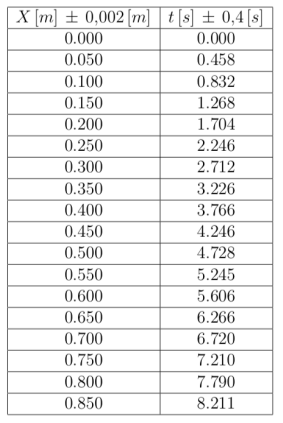
\includegraphics[width=0.8\textwidth]{tablas/tabla 6 viscosidad.PNG}
    \captionof{table}{Datos obtenidos para el Shampoo con la pelota 1, la columna t representa el promedio de las 5 distintas corridas de datos.}
    \label{fig}
\end{Figura}

\begin{Figura}
\centering
    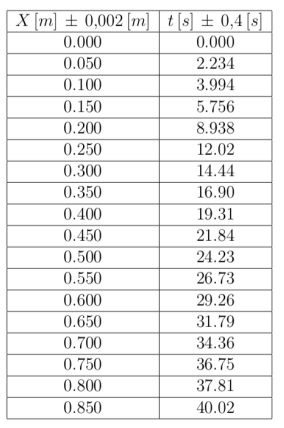
\includegraphics[width=0.8\textwidth]{tablas/tabla 7 viscosidad.PNG}
    \captionof{table}{Datos obtenidos para el Shampoo con la pelota 2, la columna t representa el promedio de las 5 distintas corridas de datos.}
    \label{fig}
\end{Figura}

\begin{Figura}
\centering
    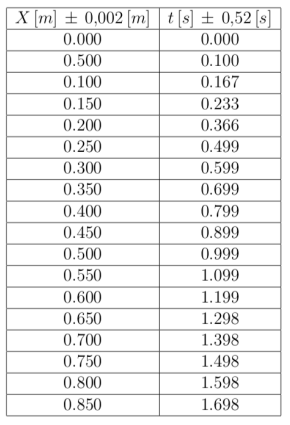
\includegraphics[width=0.8\textwidth]{tablas/tabla 8 viscosidad.PNG}
    \captionof{table}{Datos obtenidos para el agua con la pelota 2, la columna t representa el promedio de las 5 distintas corridas de datos.}
    \label{fig}
\end{Figura}

\begin{Figura}
\centering
    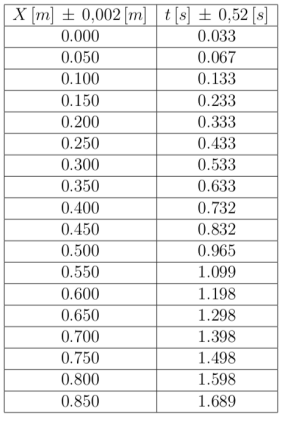
\includegraphics[width=0.8\textwidth]{tablas/tabla 9 viscosidad.PNG}
    \captionof{table}{Datos obtenidos para el agua con la pelota 3, la columna t representa el promedio de las 5 distintas corridas de datos.}
    \label{fig}
\end{Figura}

\begin{Figura}
\centering
    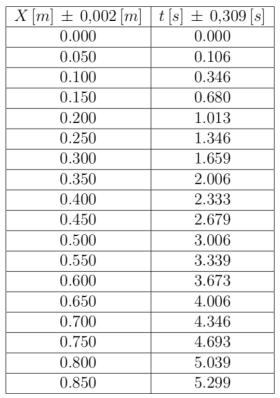
\includegraphics[width=0.8\textwidth]{tablas/tabla 10 viscosidad.PNG}
    \captionof{table}{Datos obtenidos para el glicerina con la pelota 4, la columna t representa el promedio de las 5 distintas corridas de datos.}
    \label{fig}
\end{Figura}

\end{multicols}

%\newpage


\subsection*{Densímetro}

Un densímetro o areómetro es un instrumento de medición que sirve para determinar la densidad relativa de los líquidos sin necesidad de calcular antes su masa, conductividad y temperatura. Normalmente, está hecho de vidrio y consiste en un cilindro hueco con un bulbo pesado en uno de sus extremos para que pueda flotar en posición vertical[1].

\subsection*{Modo de uso}

El densímetro se introduce verticalmente y con cuidado en el líquido, y se deja en reposo hasta que flote libre y verticalmente. A continuación, se observa en la escala graduada en el vástago del densímetro su nivel de hundimiento en el líquido; esa es la lectura de la medida de densidad relativa del líquido. En líquidos ligeros el densímetro se hundirá más que en líquidos más densos (como agua salada, leche,...). De hecho, es usual tener dos instrumentos distintos: uno para los líquidos en general y otro para los líquidos poco densos, que se diferencian en la disposición de las marcas de medida[1].

\begin{figure}
    \centering
    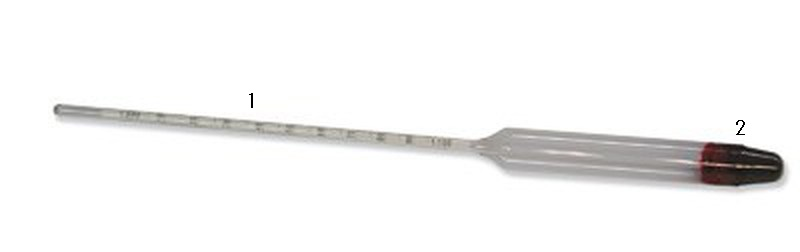
\includegraphics[scale=0.8]{densimetro.jpg}
    \caption{Densímetro: graduación (1), lastre (2).}
    \label{fig:my_label}
\end{figure}

\end{document}